\subsection{Model Training Details}

\noindent \textbf{Knowledge Distillation} \quad We conduct distillation using the method described in Distill-Bert \cite{Sanh2019DistilBERTAD}. The six distilled models we trained are named (A, B, $B_{not}$, C, D, $D_{not}$), with respectively (4,6,6,8,10,10) number of decoder blocks, as shown in Figure \ref{fig: distill}; among them, $B_{not}$ and $D_{not}$ did not use pretrained weights as initialization, while all others initialized with truncated weights from the original GPT2 model. The original training dataset of OpenAI GPT2 is the the 48GB OpenWebText. However, training on full 48GB is out of our capacity, so we randomly sampled around 1/100 of the OpenWebText data to train the distilled models. Training takes 3 epochs, and it automatically saves the best performing model; The other training hyper-parameters are the same as the GPT-2 Model in huggingface. The average training time is 6 hours on 2 A100 GPUs, and the smaller the student model, the faster the training. The perplexity of trained models is shown in Figure \ref{fig: ppl}.\\

\begin{figure}[ht]
% 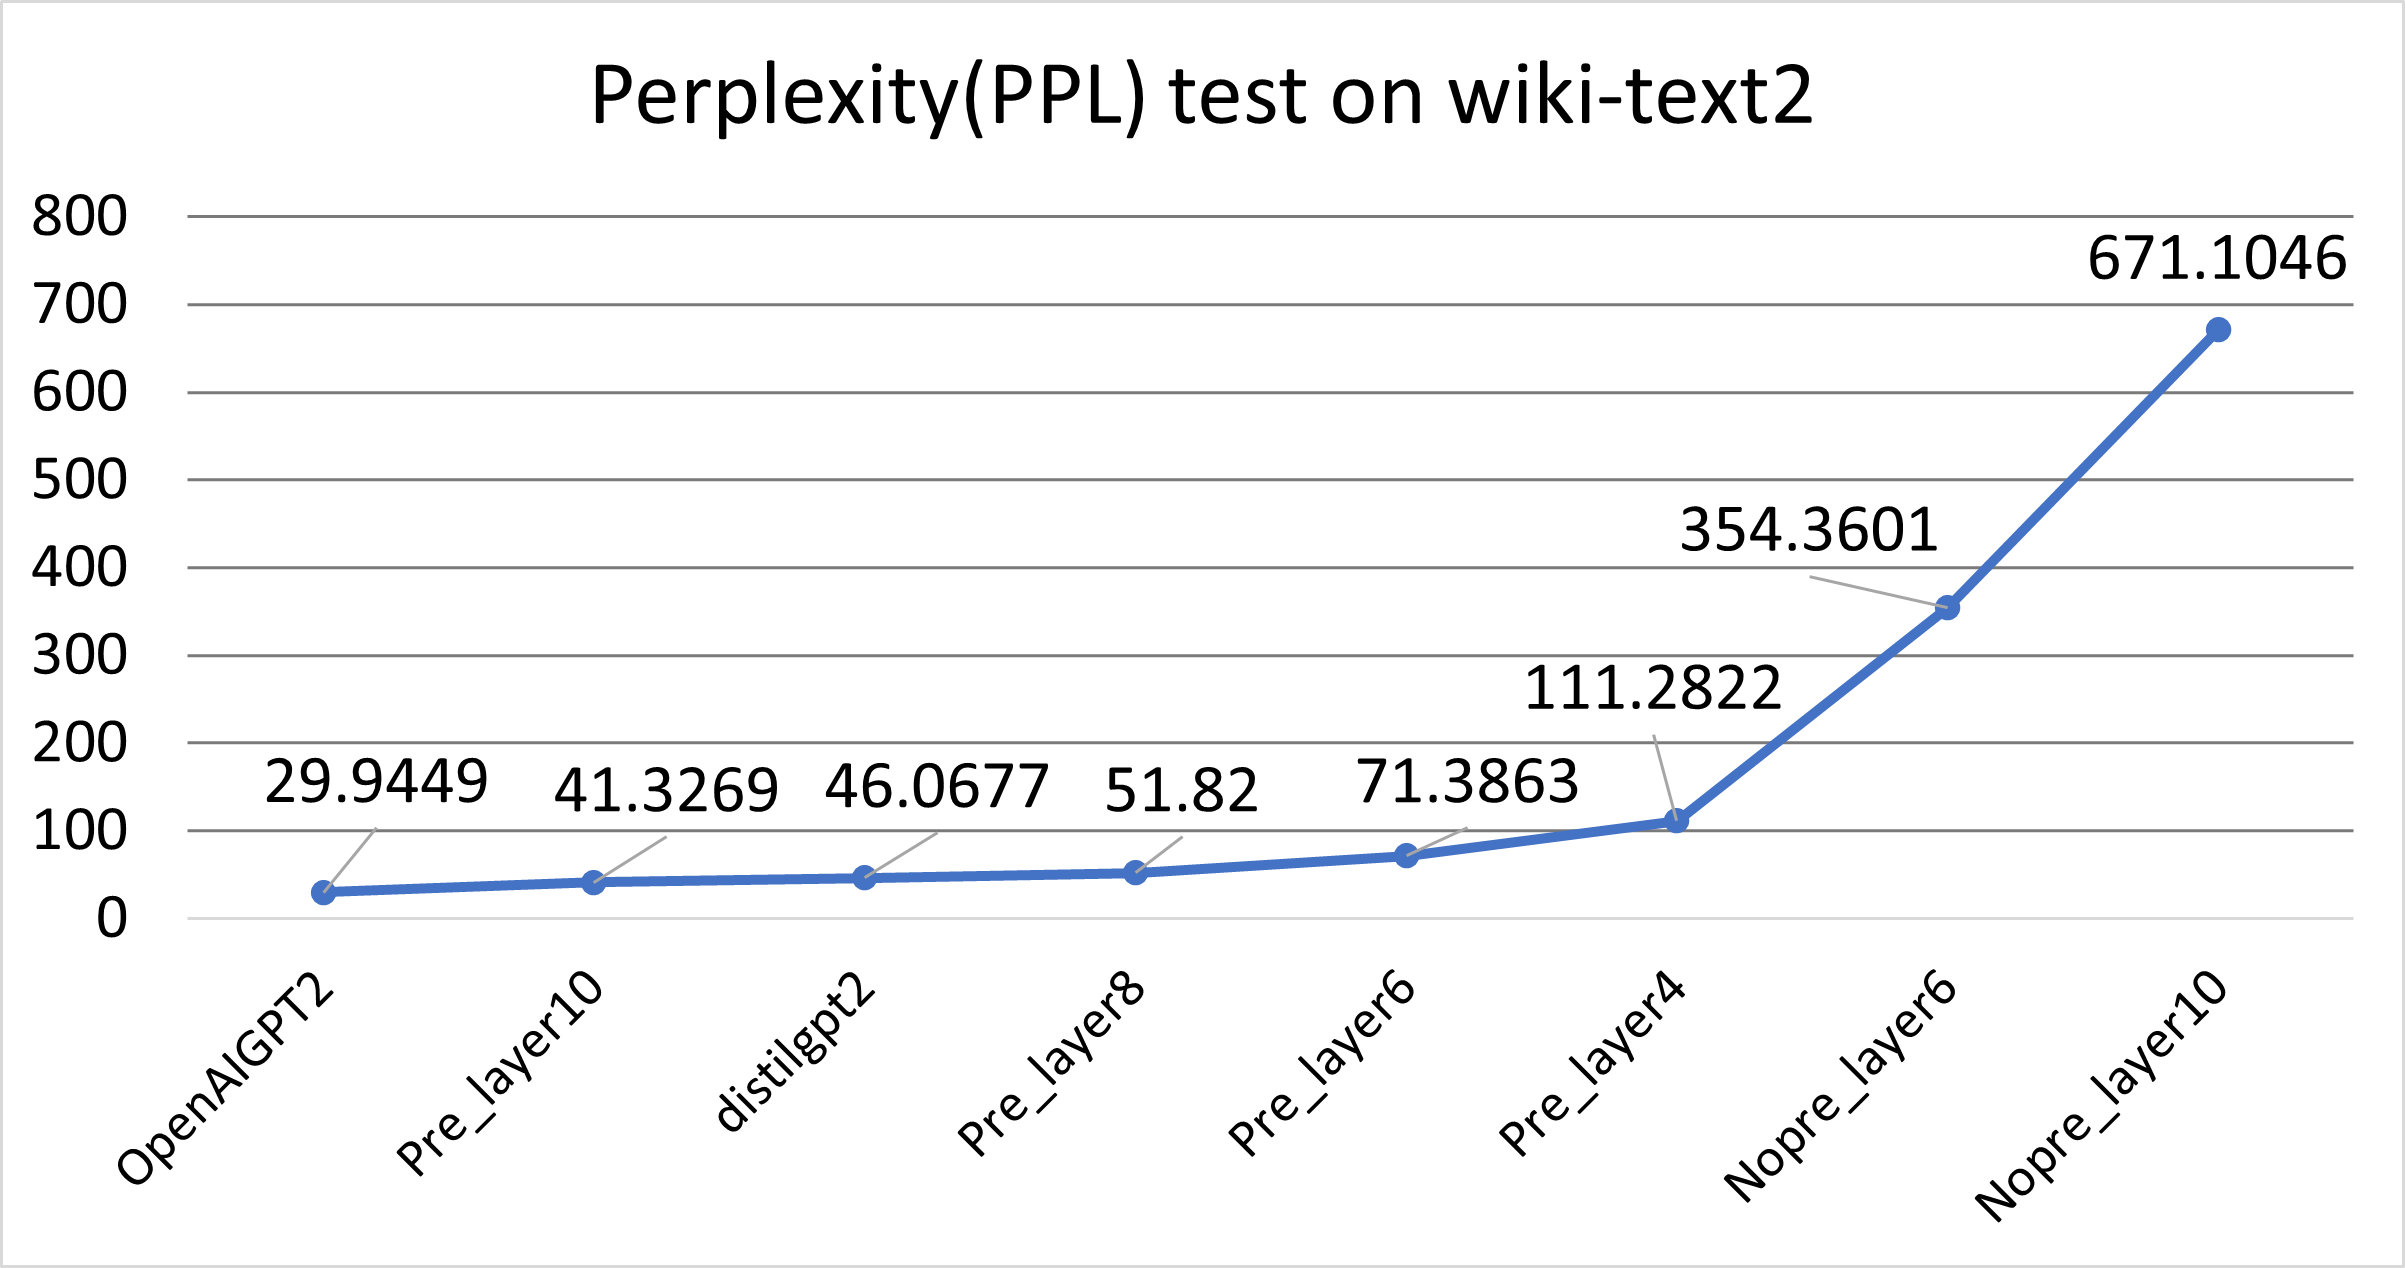
\includegraphics[width=7.5cm, height=4cm]{graphs/distill_ppl.png}
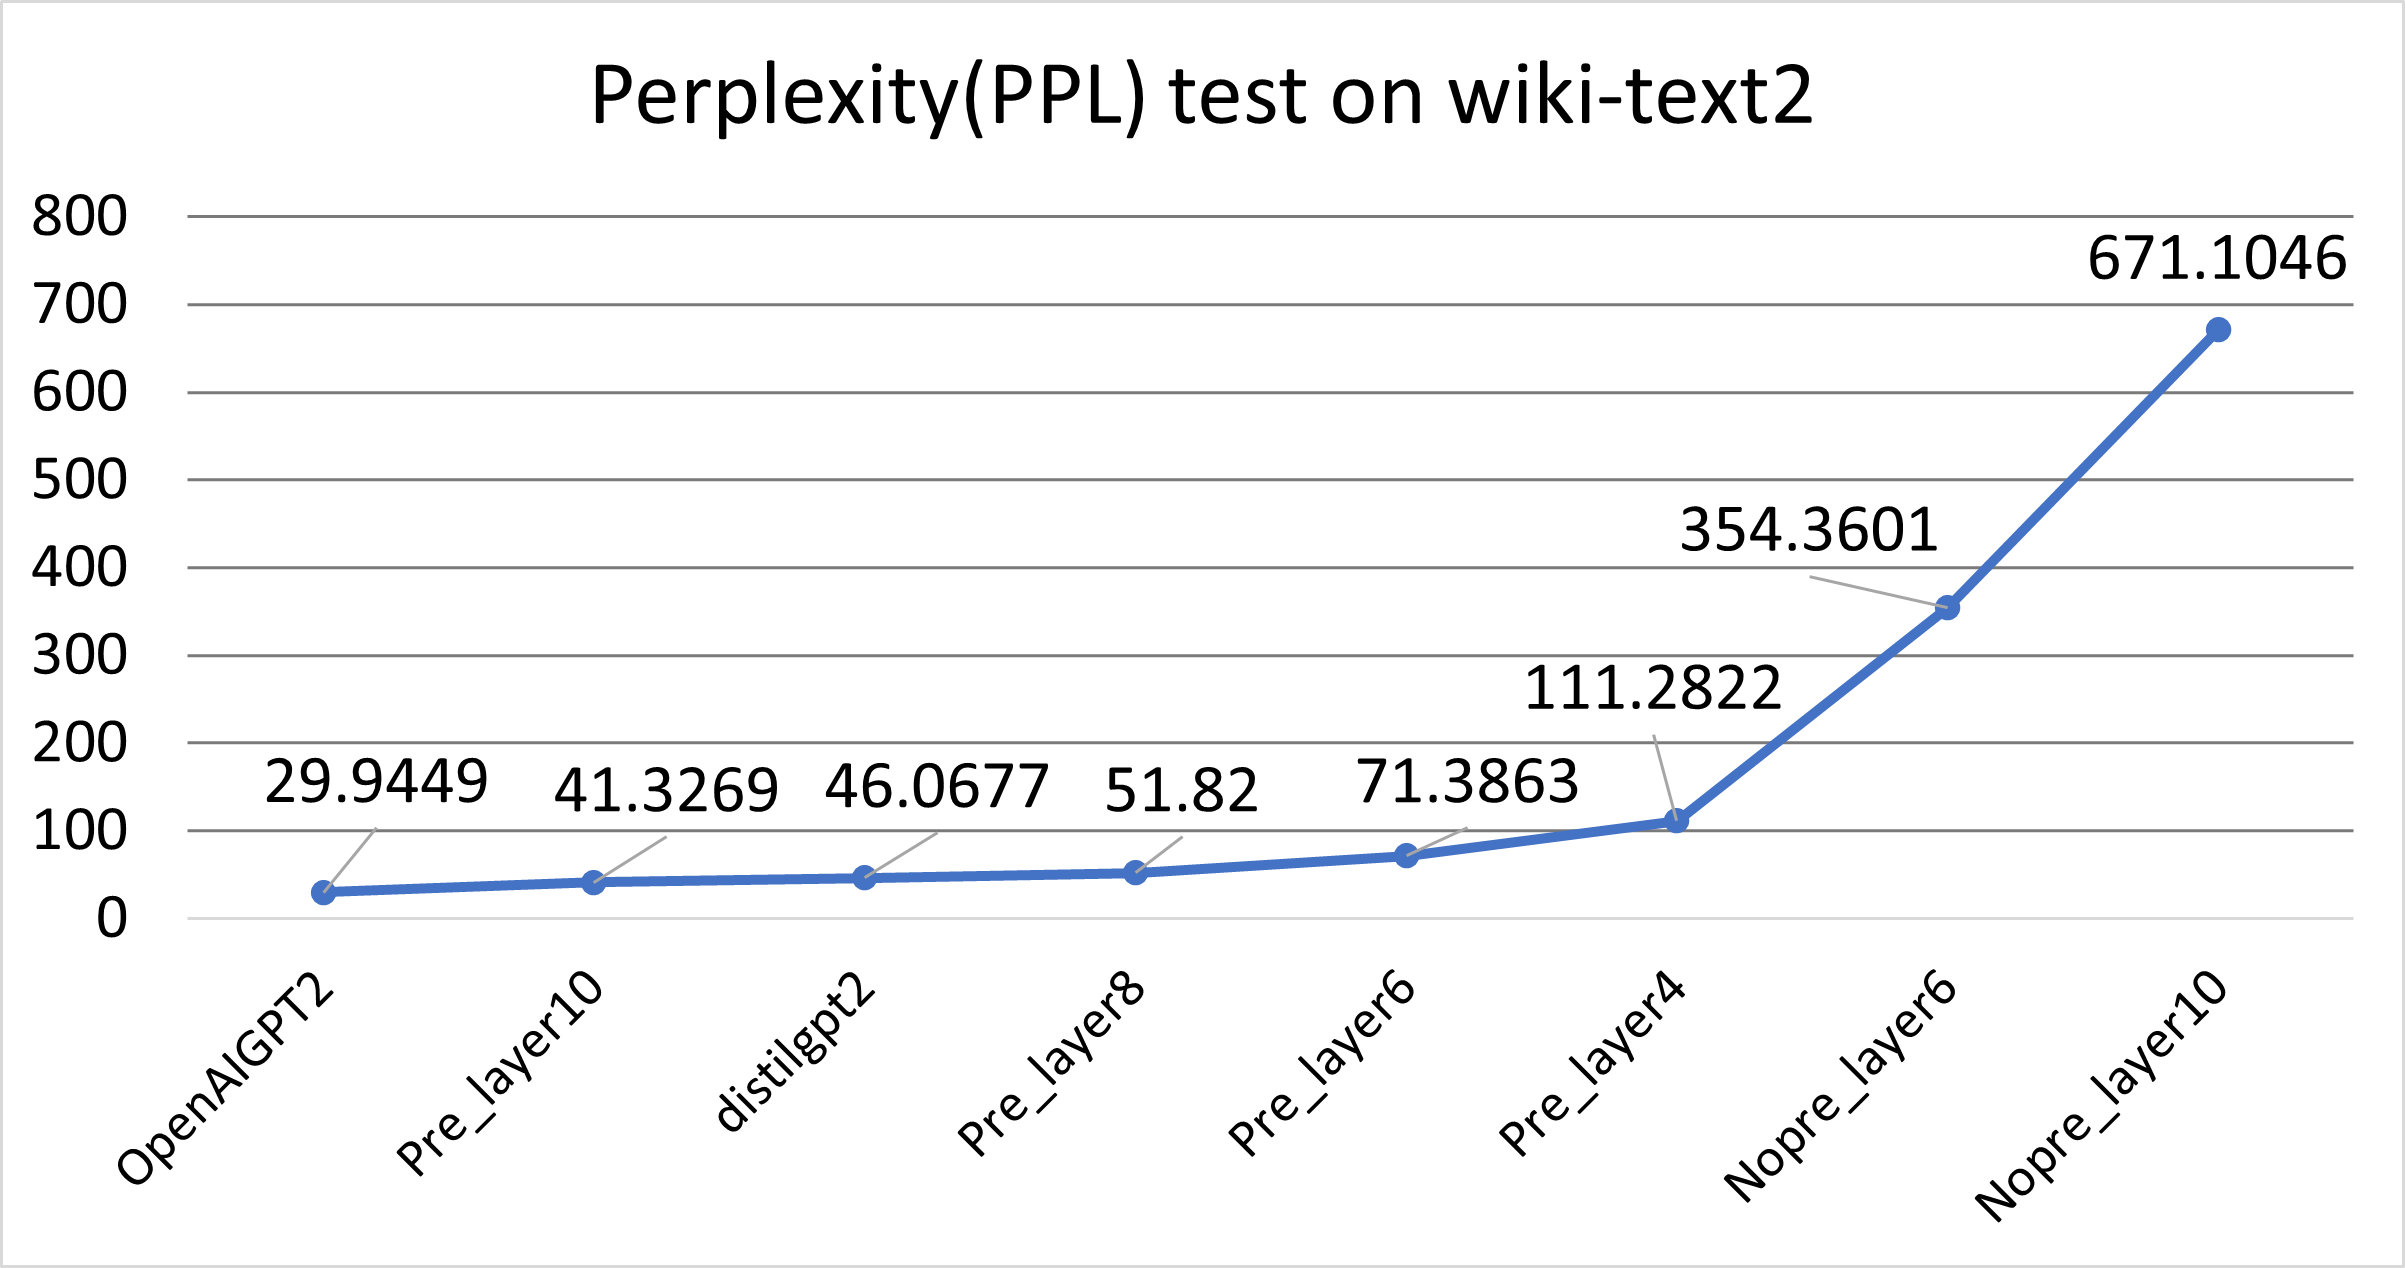
\includegraphics[scale = 0.4]{graphs/distill_ppl.png}
\caption{Perplexity of distilled models}
\centering
\label{fig: ppl}
\end{figure}


\noindent \textbf{Pruning} \quad Pruning applies the method proposed in \cite{Michel2019AreSH}. We start with pretrained GPT2 model from HuggingFace which has 144 attention heads in total. In each prune iteration, we sort the heads by a proxy importance score and mask the lowest important 5 percent. And we repeat the pruning 3 times which results in keeping 85 percent of the heads. We choose to use WikiText which contains a reasonable number of data (~35K). In this experiment, we sample 5 subsets with various sizes from the WikiText and conduct pruning using these subsets, namely 256, 1280, 2560, 5120, and 12800. They all have the same size, and report their perplexity (PPL) score along with the original model in Figure \ref{fig: prune_ppl}. As a result of the pruning, we observed 1.2x to 1.5x computation speed improvement. We observe that using a larger dataset as validation can help improve the pruning performance, as expected, since larger datasets results in more representative proxy importance scores.

%As illustrated in Figure \ref{fig: prune_ppl}, the results show that, the PPL of the pruned models decreases as the size of the data increases. For example, PPL of the model using 12800 data samples is significantly smaller than the model with 256 samples. Further for sample sizes with more than 1280, we don't observe obvious decrease of the PPL. This could imply that a small subset of the dataset (1280 out of ~35000) is sufficient to prune a model without loosing performance. If this observation stands, the pruning can be significantly accelerated. Moreover, comparing with the pretrained model which scored 29.9, both the PPL of pruned models and the distilled model have similar but higher values. 

\begin{figure}[ht]
% 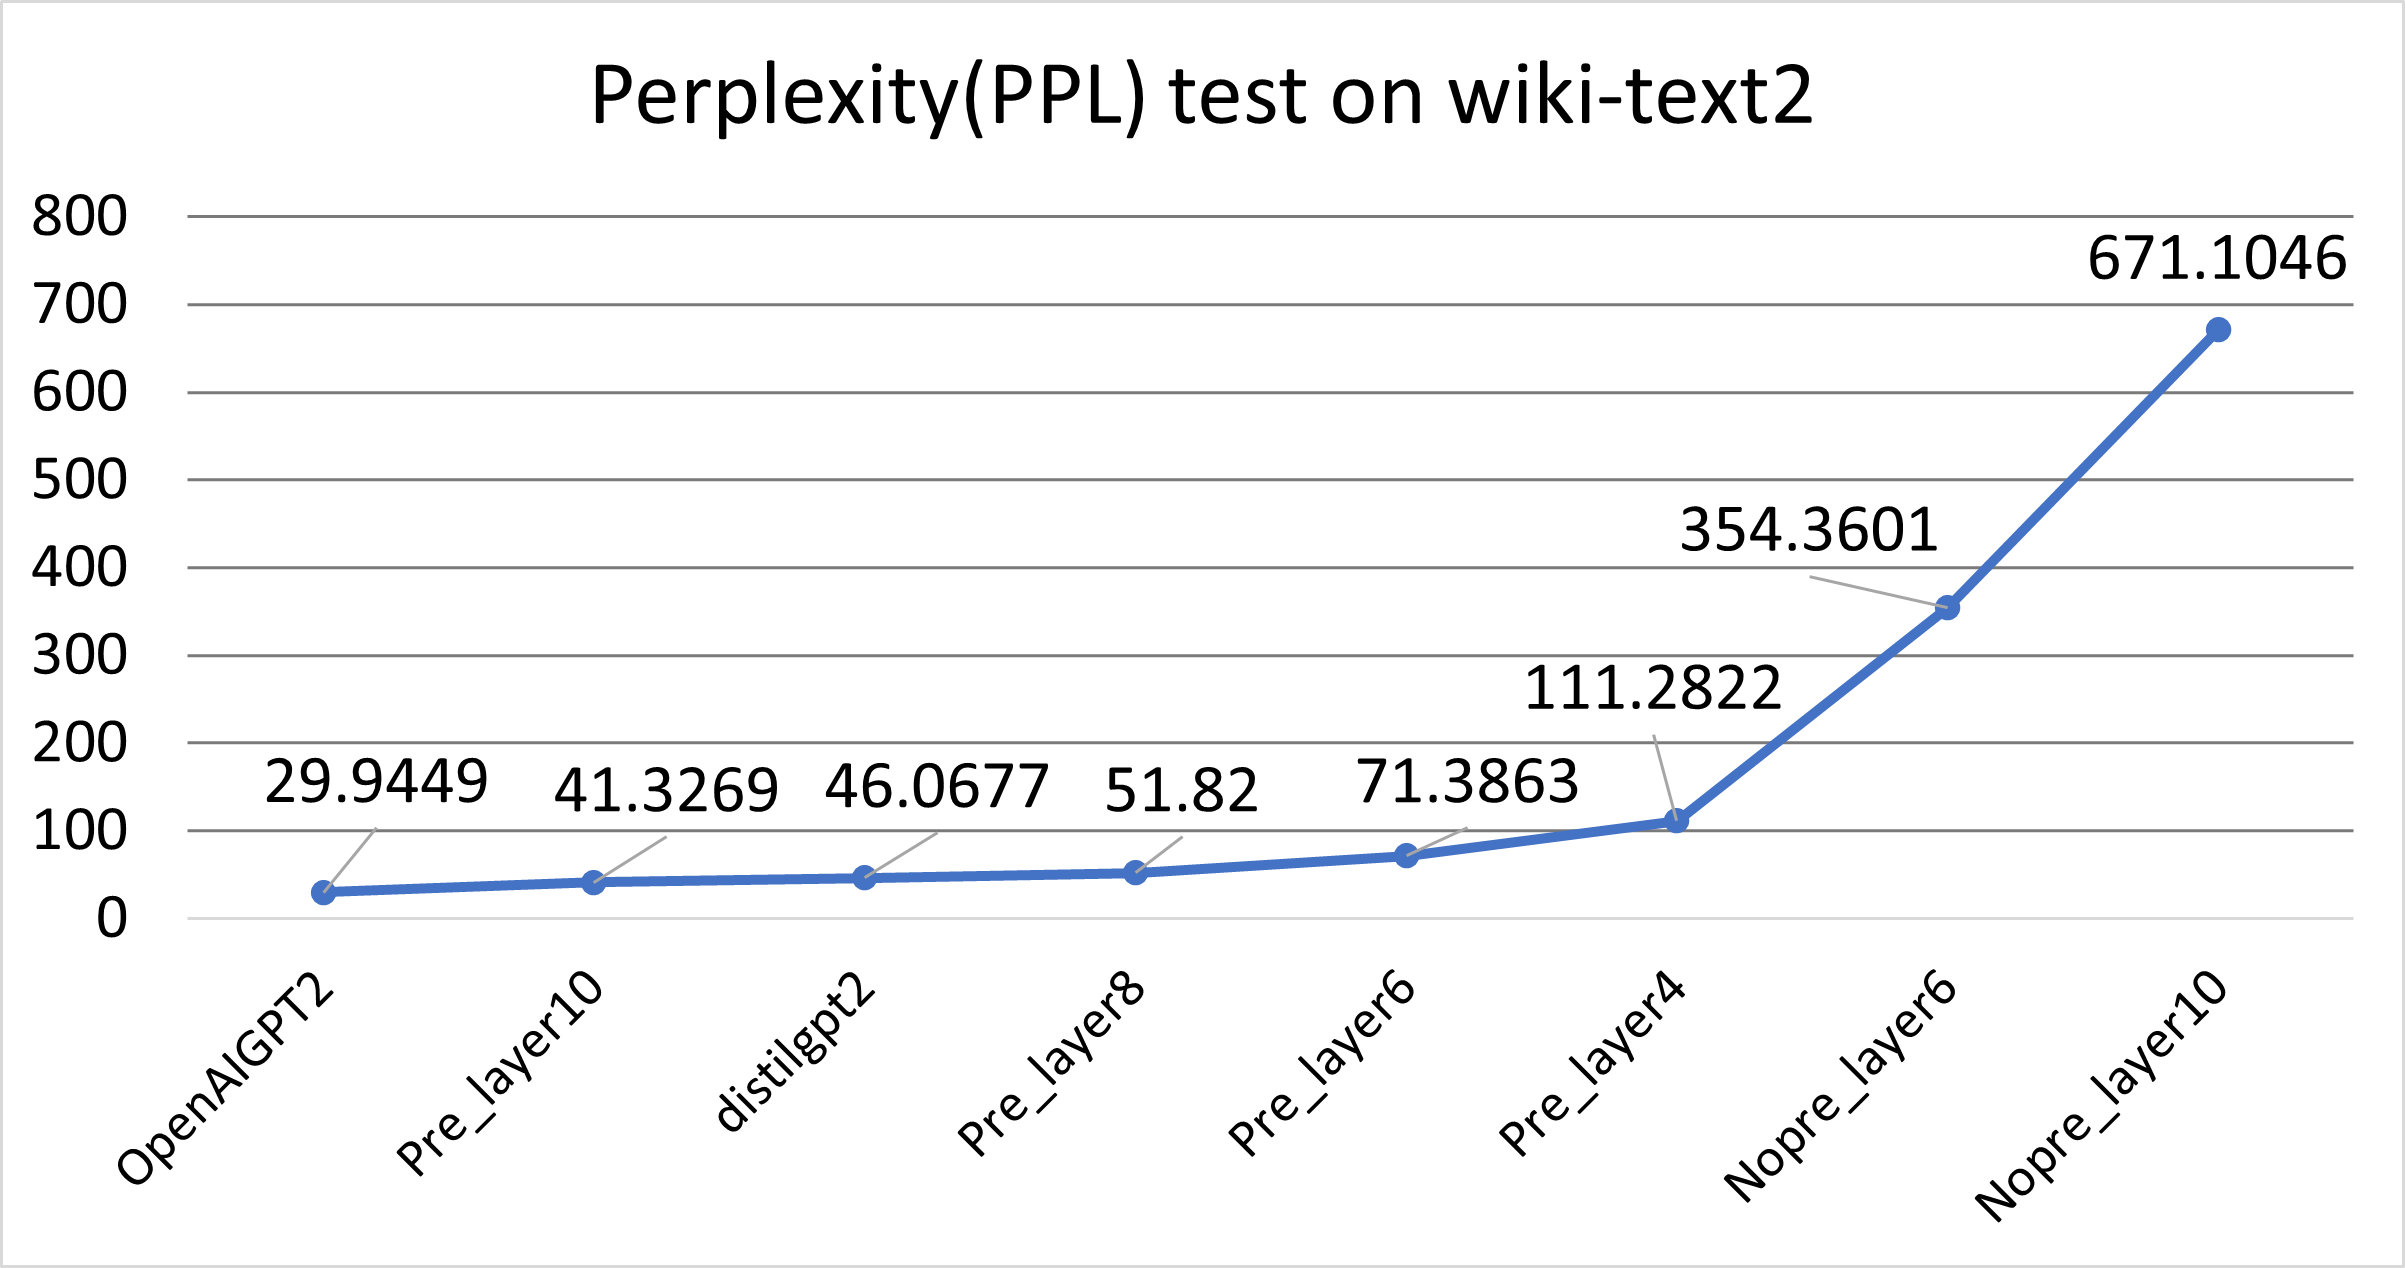
\includegraphics[width=7.5cm, height=4cm]{graphs/distill_ppl.png}
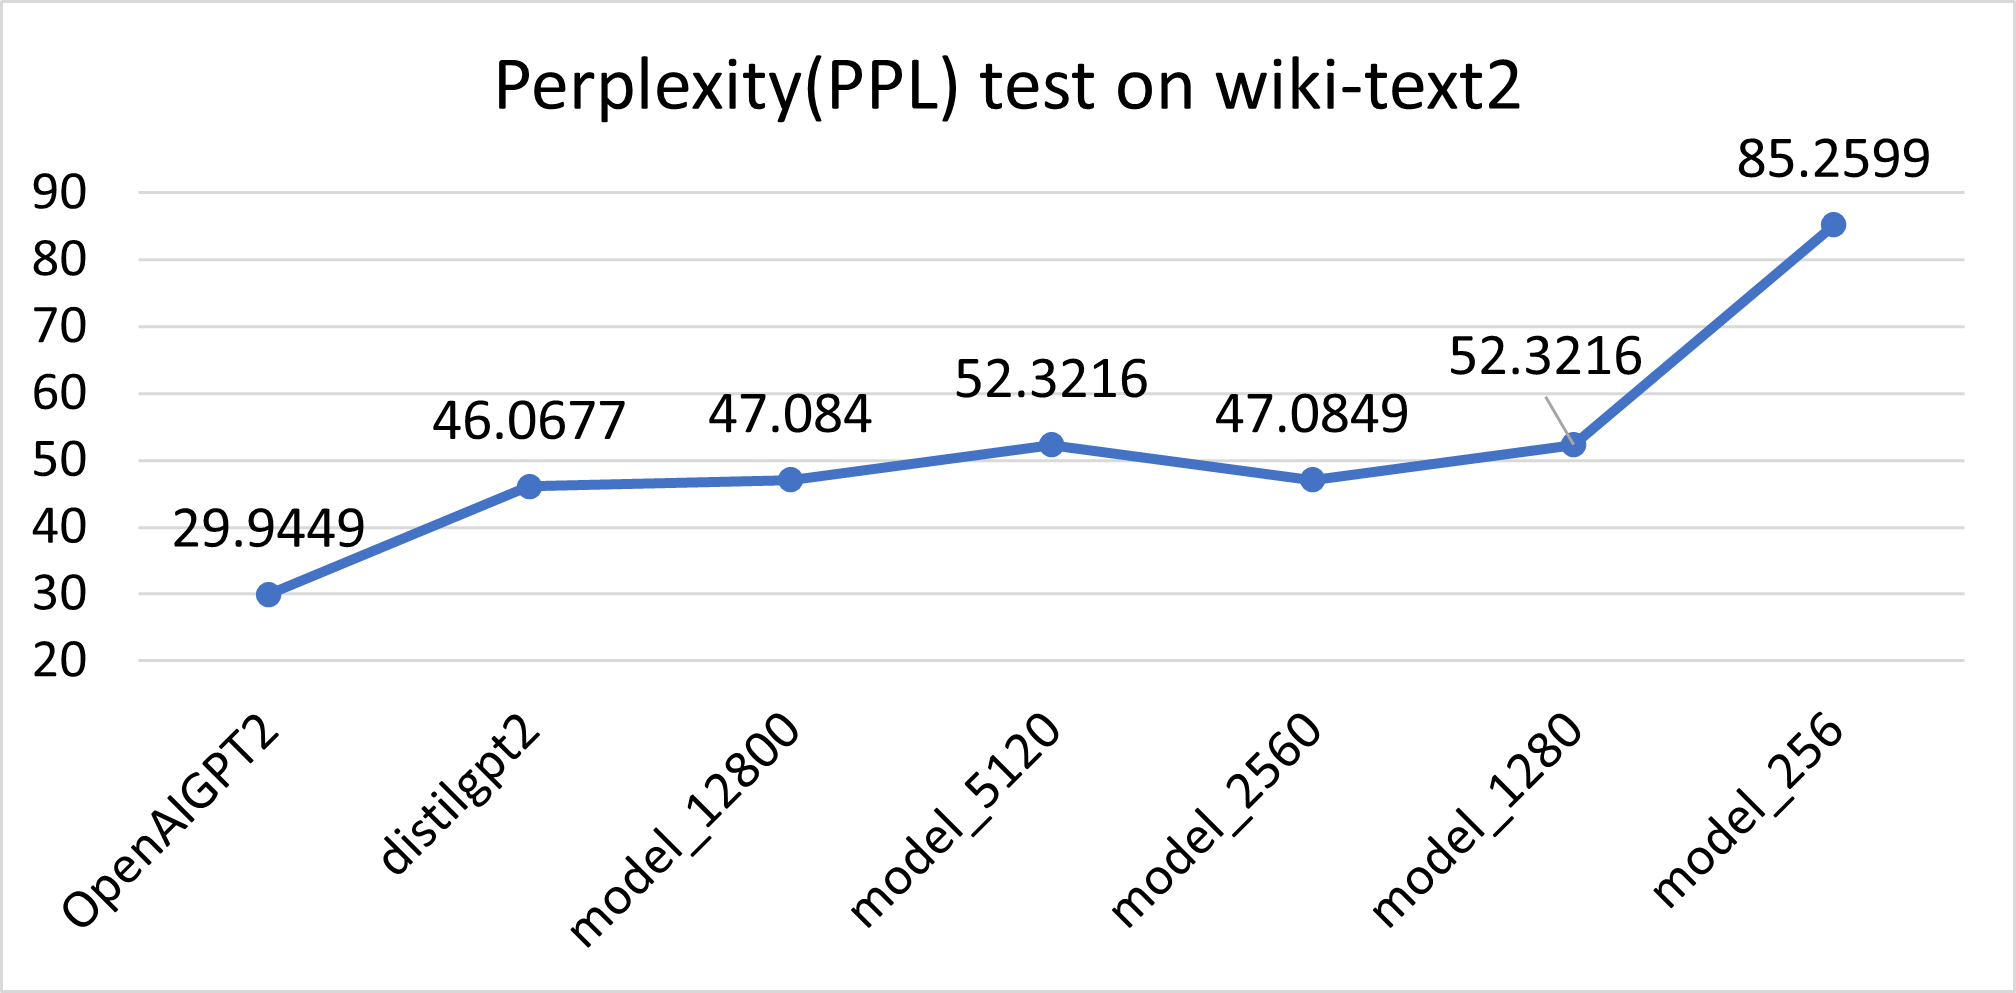
\includegraphics[scale = 0.48]{graphs/prune_ppl.png}
\caption{Perplexity of pruned models}
\centering
\label{fig: prune_ppl}
\end{figure}

\begin{figure*}[ht]
% 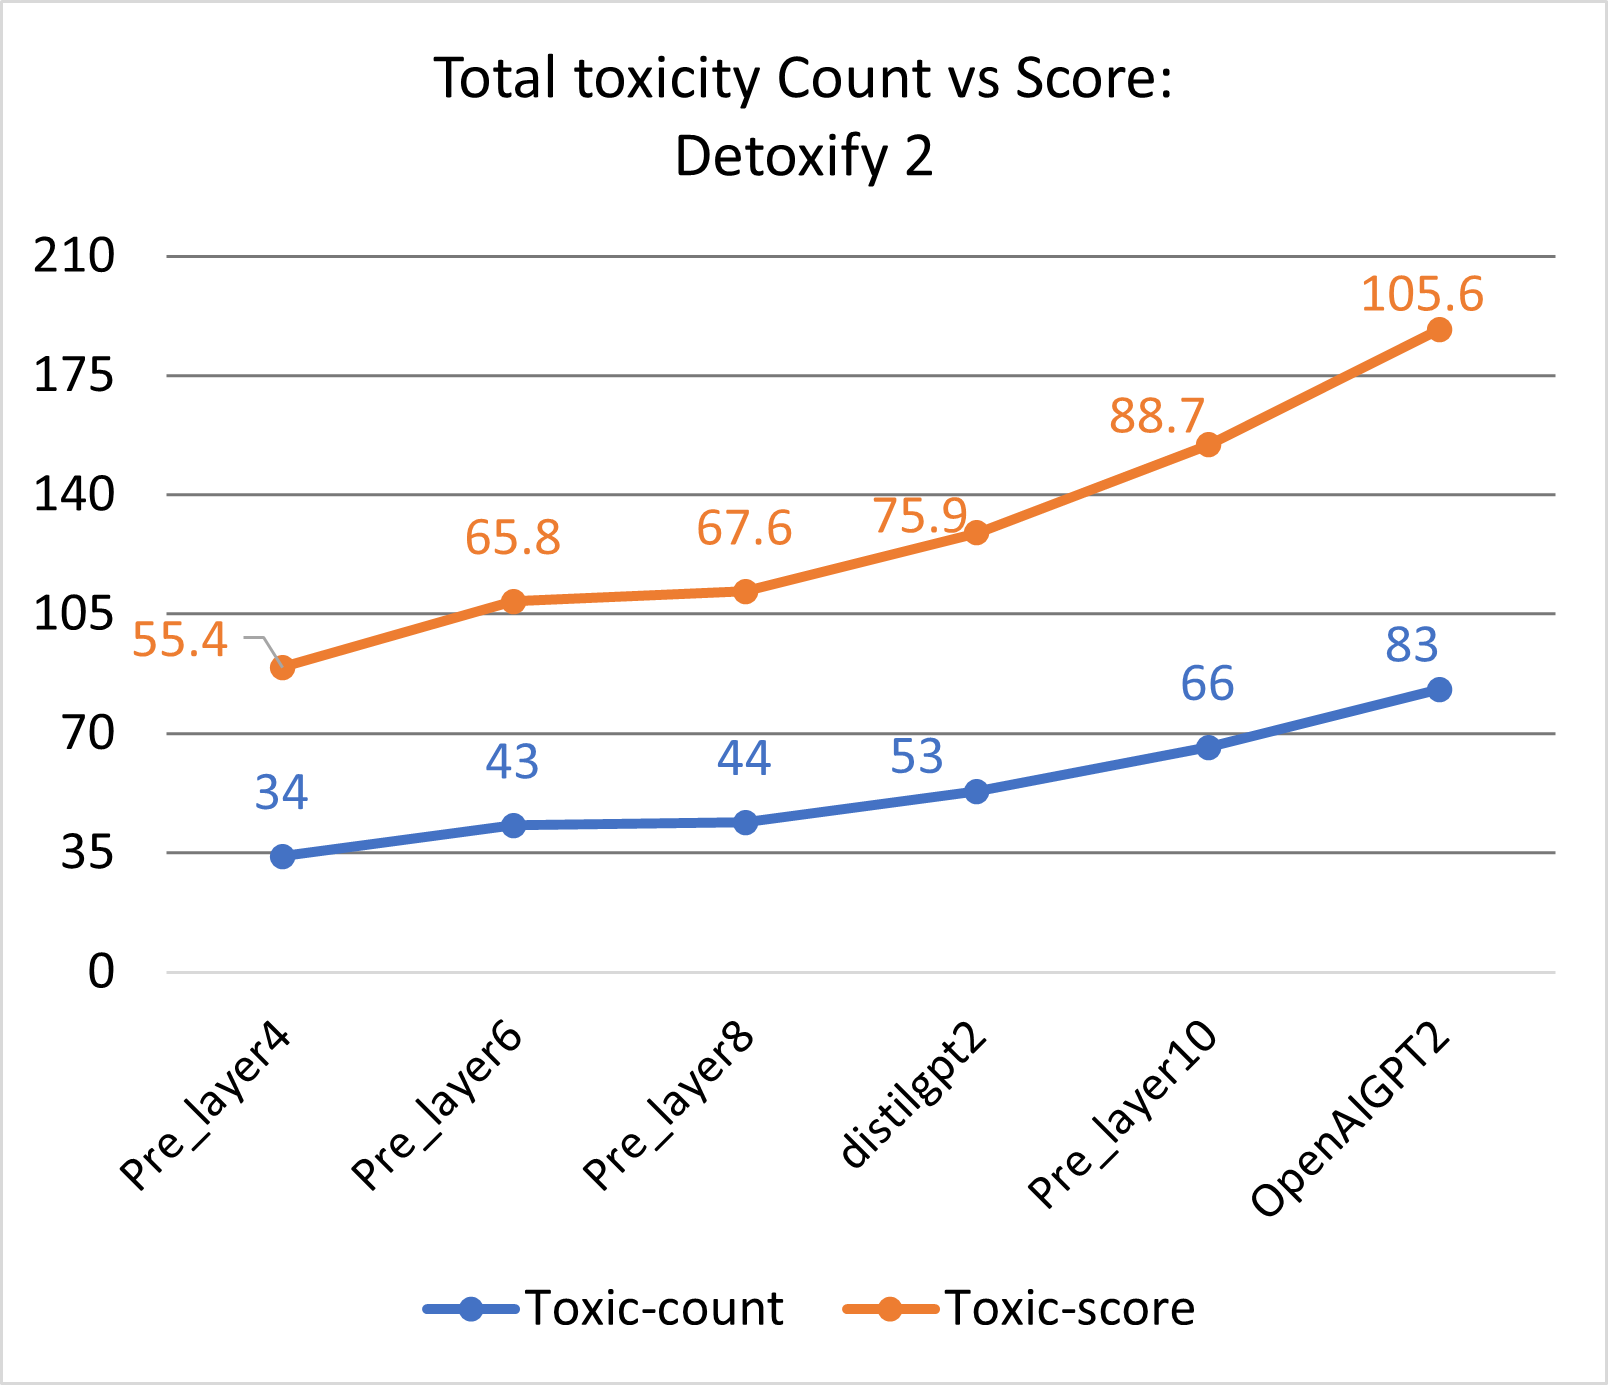
\includegraphics[width=7.5cm, height=5.5cm]{graphs/detoxify2.png}
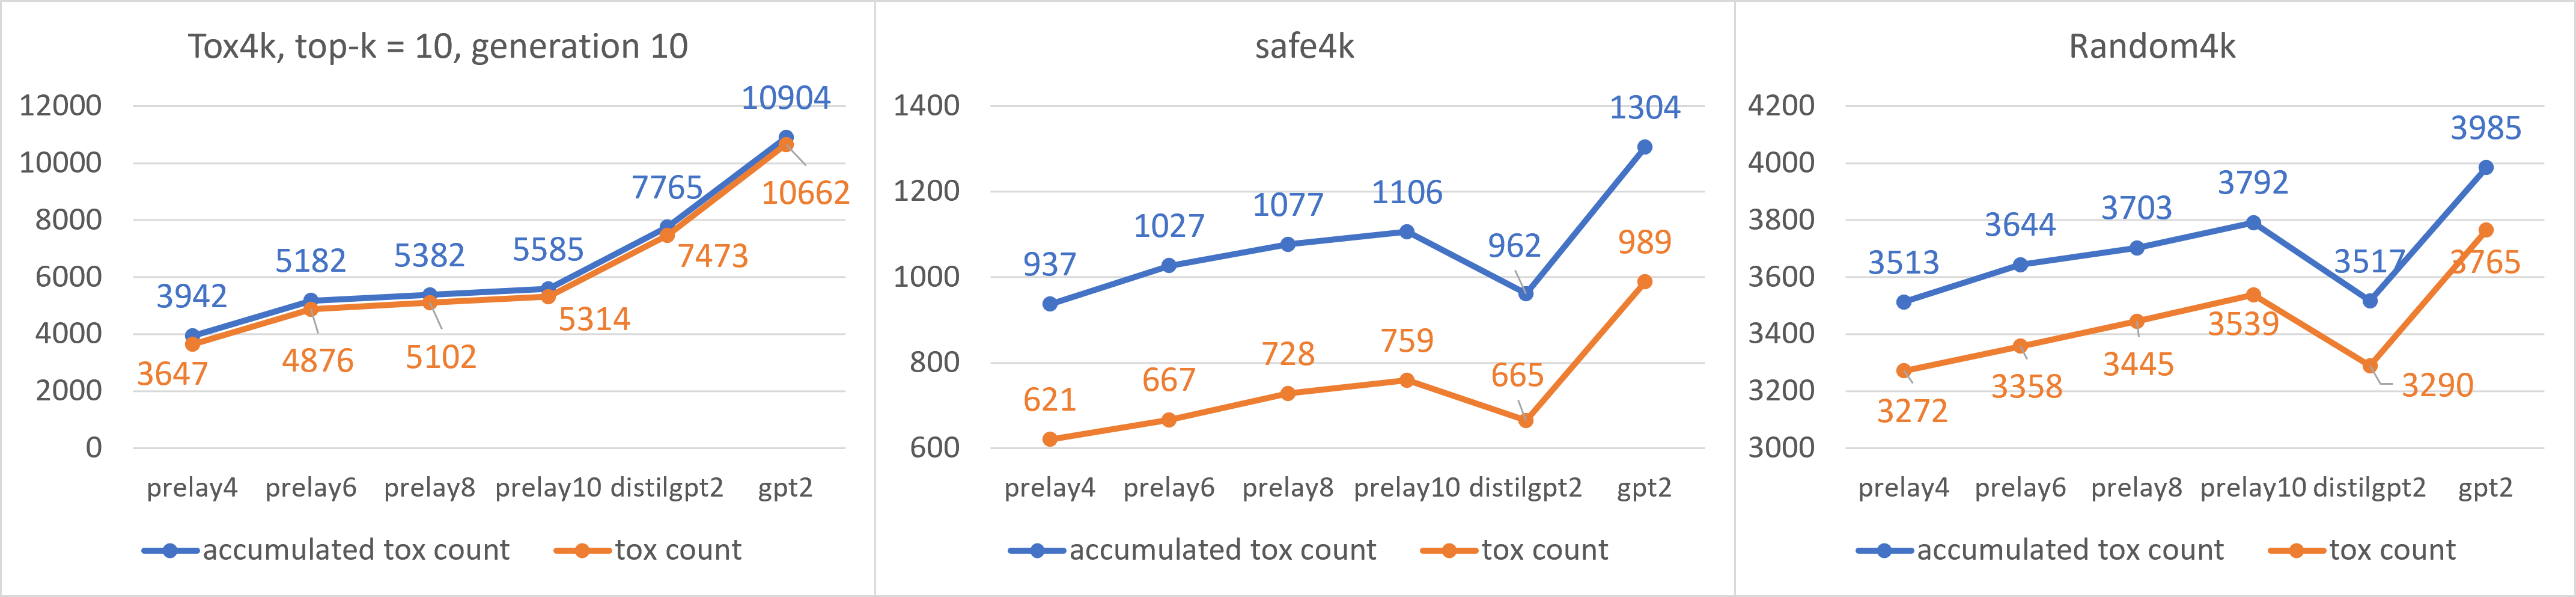
\includegraphics[width = \textwidth]{graphs/tox_random_safe.png}
\caption{Toxicity tested on TCCC }
\centering
\label{fig: tox_random_safe}
\end{figure*}

\subsection{Toxicity in Model Generation}
\noindent \textbf{Experiment Setup} \quad(Note that the following experiments are all conducted on Knowledge Distillation Models, because we do not have enough usable pruned models yet.) Using two prompt datasets, RealToxicityPrompts \cite{Gehman2020RealToxicityPromptsEN} and the Toxic Comments Classification Challenge(TCCC) , we run generation with different generative models and note their respective toxic count and toxic score; all models uses top-k search = 10, sample=True; as described in the previous section, we use Detoxify classifier to detect toxic examples, counting the total number of samples with toxic probability over 0.5(toxic count), and calculating the accumulated toxic probability of all samples(toxic score). For both datasets, we tried different sampling strategies, and produced the toxicity plot of different models under those settings.\\



\noindent \textbf{RealToxicityPrompts} \quad For this dataset, we sampled 1200 toxicity triggers, which are non-toxic prompts but leads to toxic continuation in the actual data. Each model generates three sentences for each prompt, so, we are evaluating 3600 sentences per model. The toxicity level in the model generation is illustrated in Figure \ref{fig: real}. Note that RealToxicityPrompts is sourced from the training dataset of GPT2, which means the GPT2 model has seen those toxic prompts before. If the GPT2 models seems very toxic in this setting, the reason may lie in its memorization of toxic training data: distilled models are heavily regularized and less likely to output the toxic training data than the GPT2 model.\\

\begin{figure}[h]
% 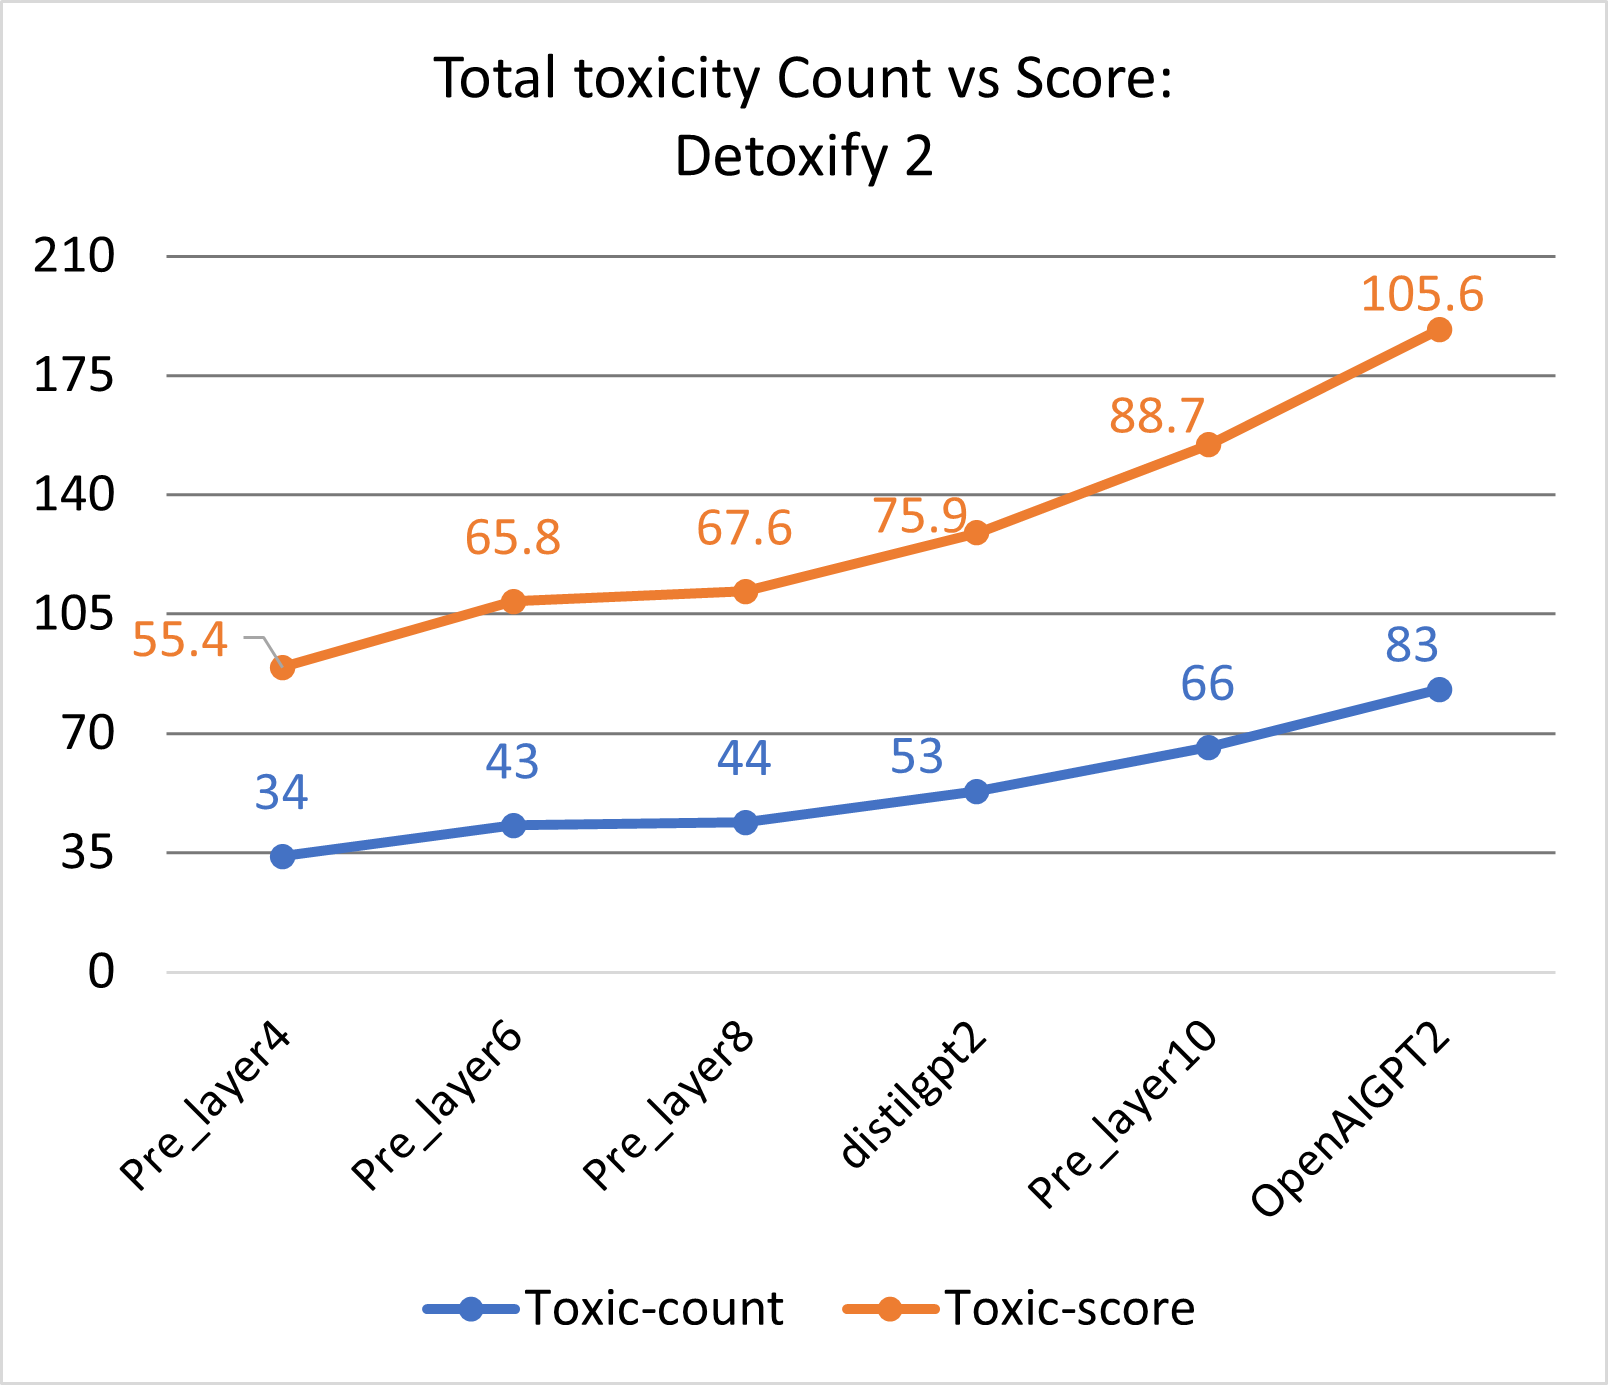
\includegraphics[width=7.5cm, height=5.5cm]{graphs/detoxify2.png}
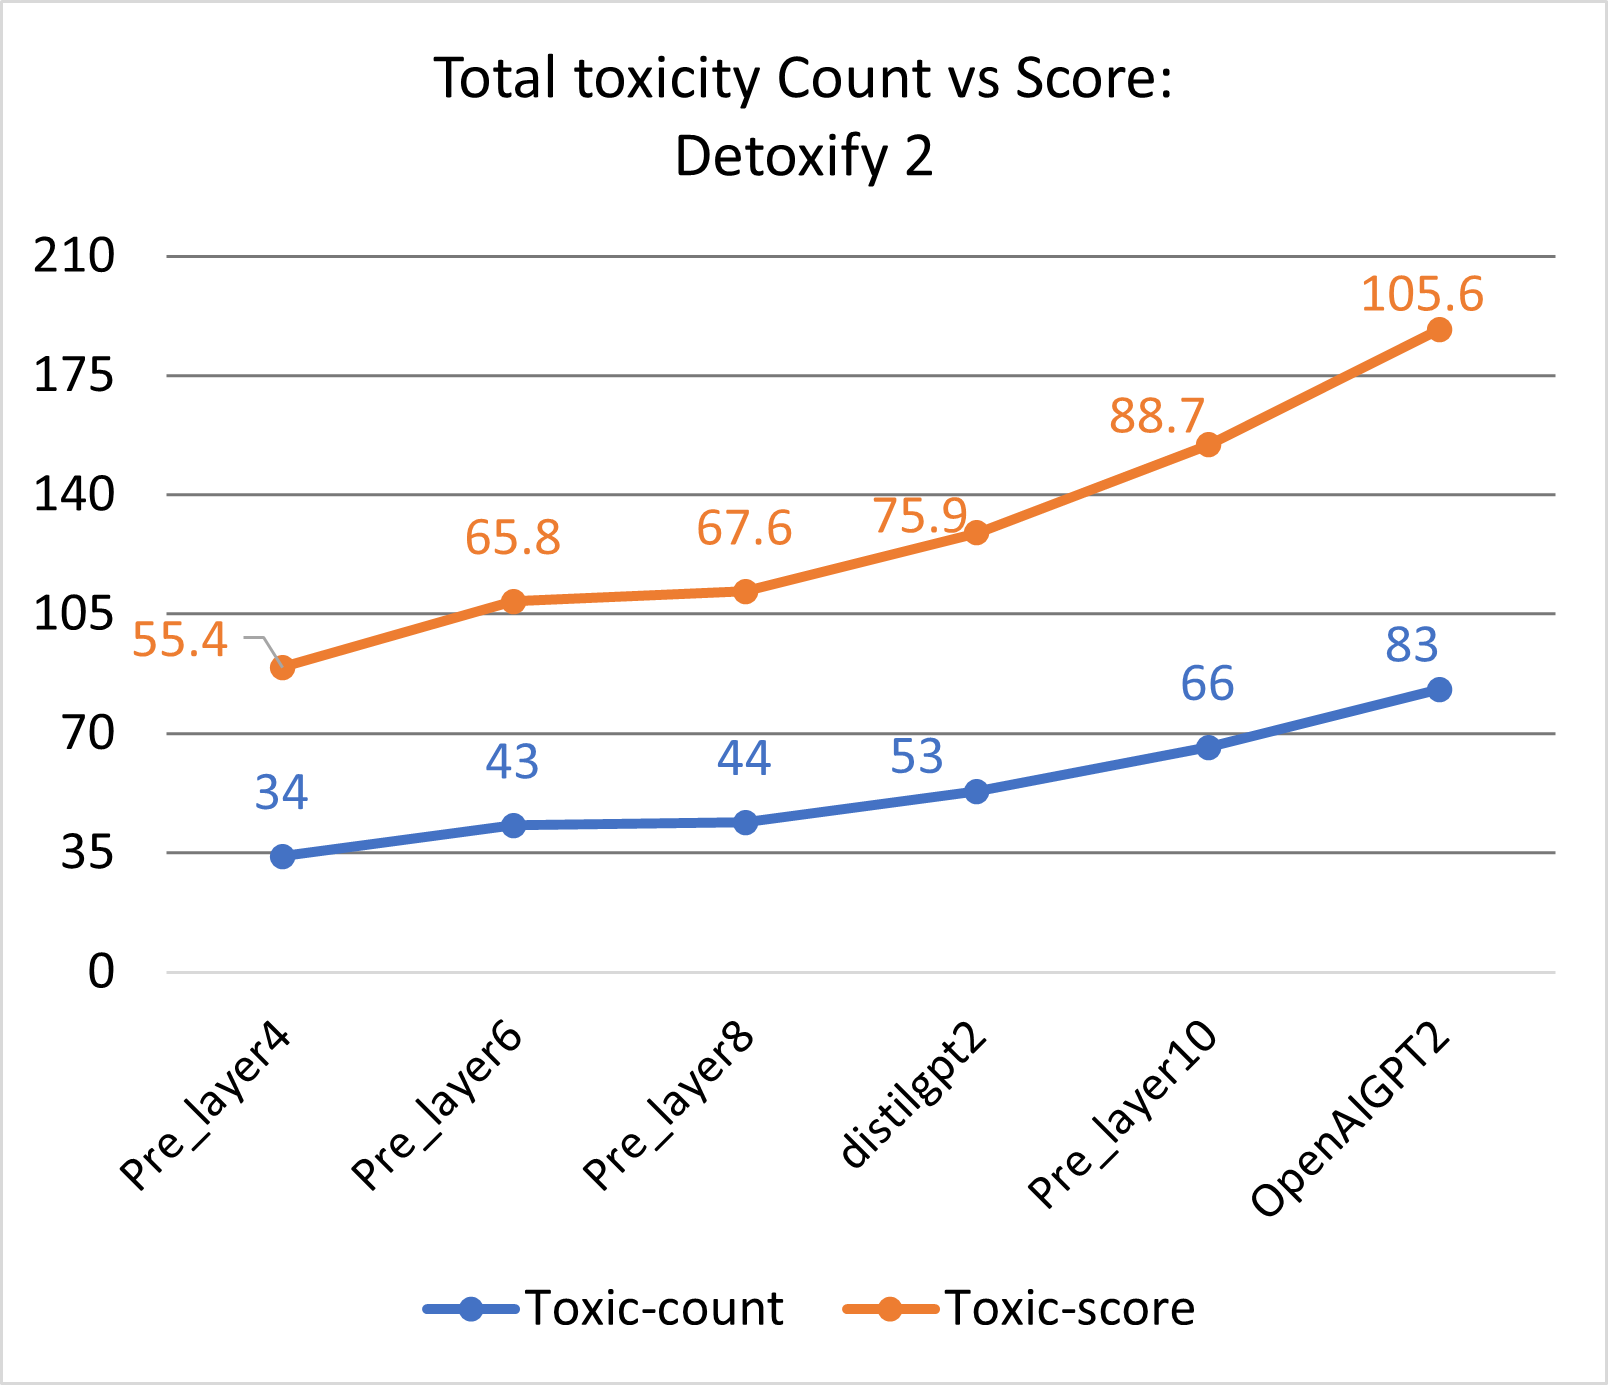
\includegraphics[scale = 0.6]{graphs/detoxify2.png}
\caption{Real Toxicity Prompts}
\centering
\label{fig: real}
\end{figure}

\noindent \textbf{TCCC Prompts} \quad Different from the RealToxicityPrompts dataset, GPT2 has never trained on the TCCC dataset. And we adopted three sampling strategies to build three test datasets, each containing 4k samples, named as(tox4k, random4k, safe4k). The tox4k contains prompts cropped from originally toxic sentences; the random4k's prompts are cropped from randomly sampled sentences in TCCC, in which around 10 percent data is toxic; the safe4k's prompts are cropped from very safe sentences, with toxic score lower than 0.001. The Figure \ref{fig: tox_random_safe} illustrate the toxicity distribution of different models under different sampling settings. To note, toxicity detection is performed on full sentence for random4k and safe4k; but only the generated part is rendered for toxicity detection in tox4k, because otherwise, all samples will be found toxic.\\


\begin{table}[hb]
\centering
\begin{tabular}{|c|c|c|c|}
\hline
            & Tox4k   & Random4k & Safe4k  \\ \hline
prelay4     & 93.7  & 110.7  & 113.3 \\ \hline
prelay6     & 91.8  & 108.4  & 110.9 \\ \hline
prelay8     & 90.4  & 107.8  & 109.6 \\ \hline
prelay10    & 89.4  & 107.6  & 110.1 \\ \hline
distillgpt2 & 165.3 & 174.9  & 175.6 \\ \hline
gpt2        & 185.2 & 197.5  & 199.0 \\ \hline
\end{tabular}
\caption{Average Length of Generation}
\centering
\label{fig: length}
\end{table}


\noindent \textbf{Observation} \quad We observe that toxicity level consistently decrease as the model size becomes smaller, in all 4 depicted sampling settings, and in two different toxicity evaluation dataset. 

\begin{figure}[ht!]
% 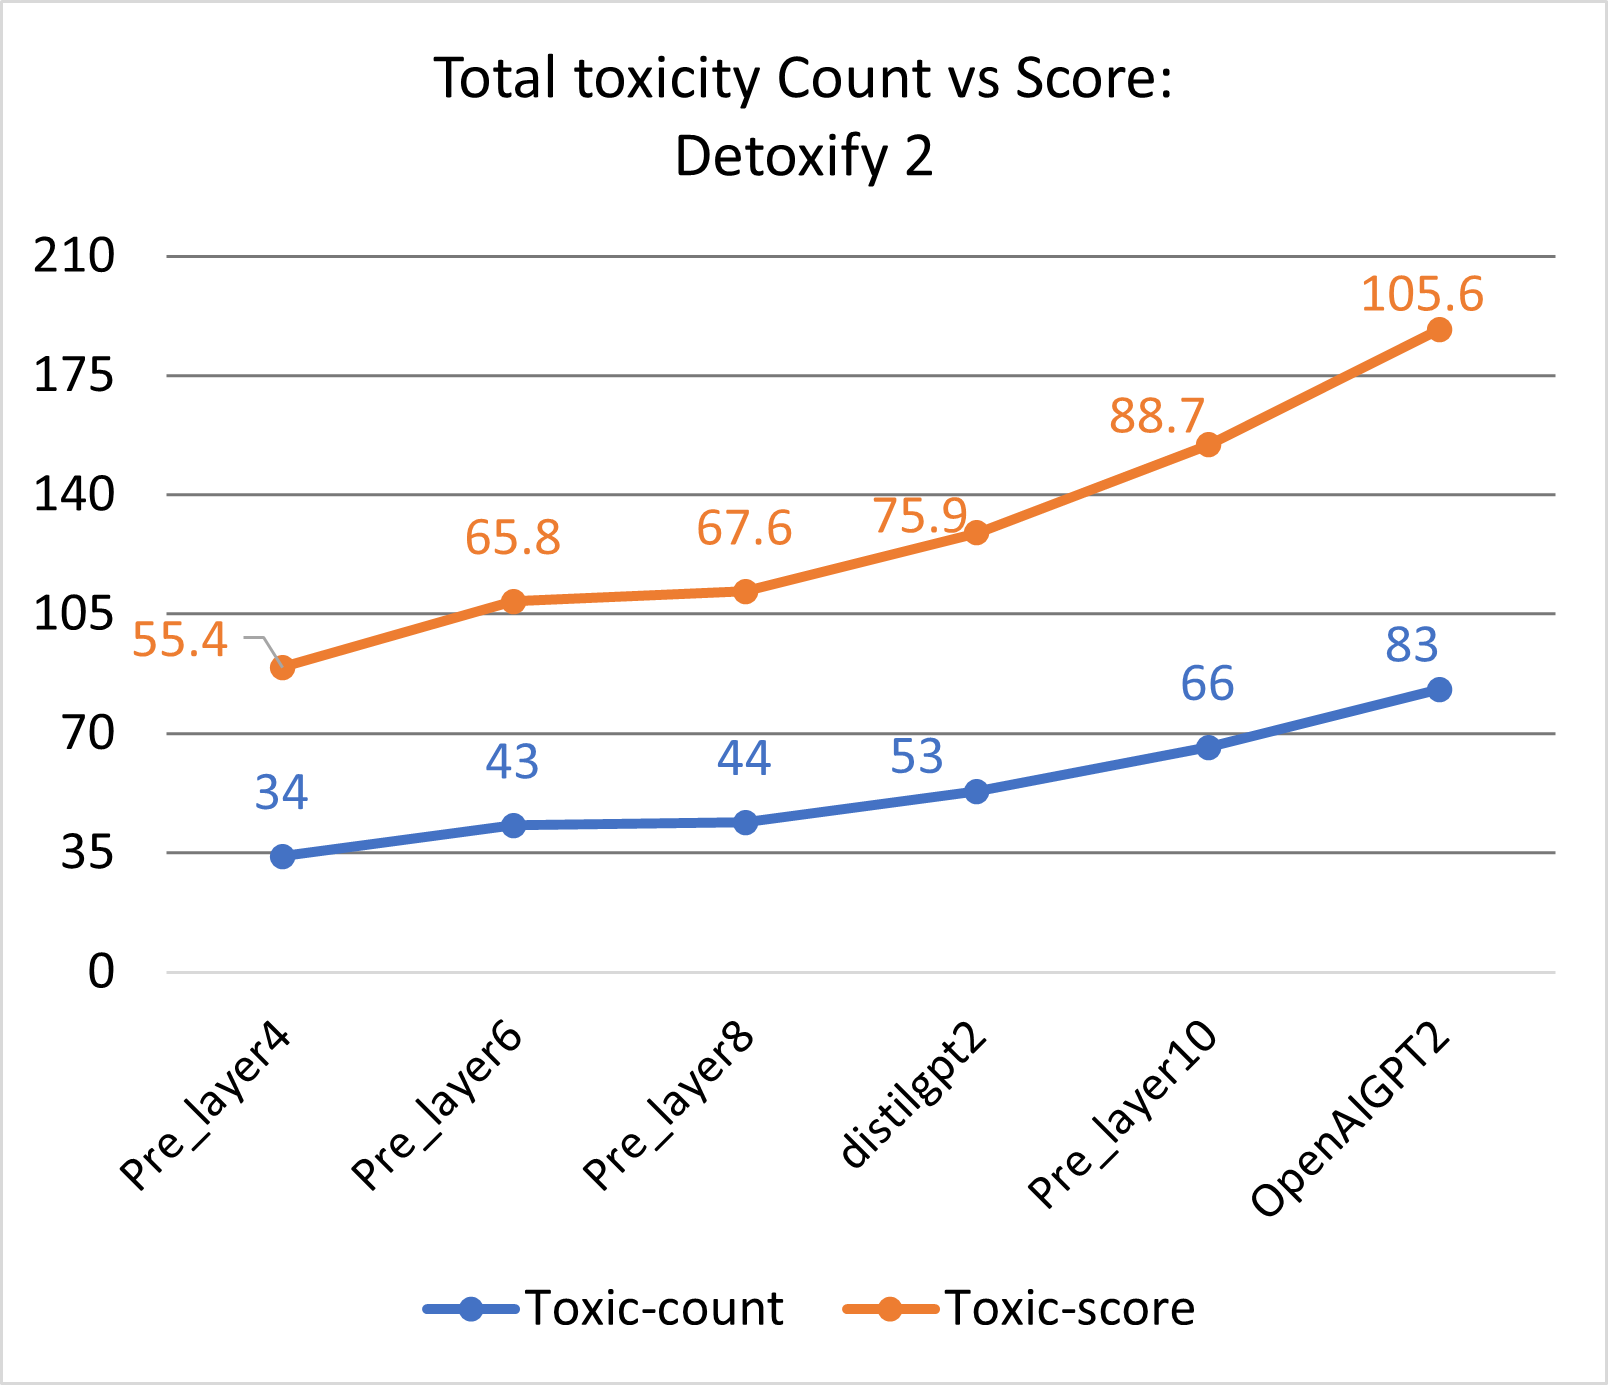
\includegraphics[width=7.5cm, height=5.5cm]{graphs/detoxify2.png}
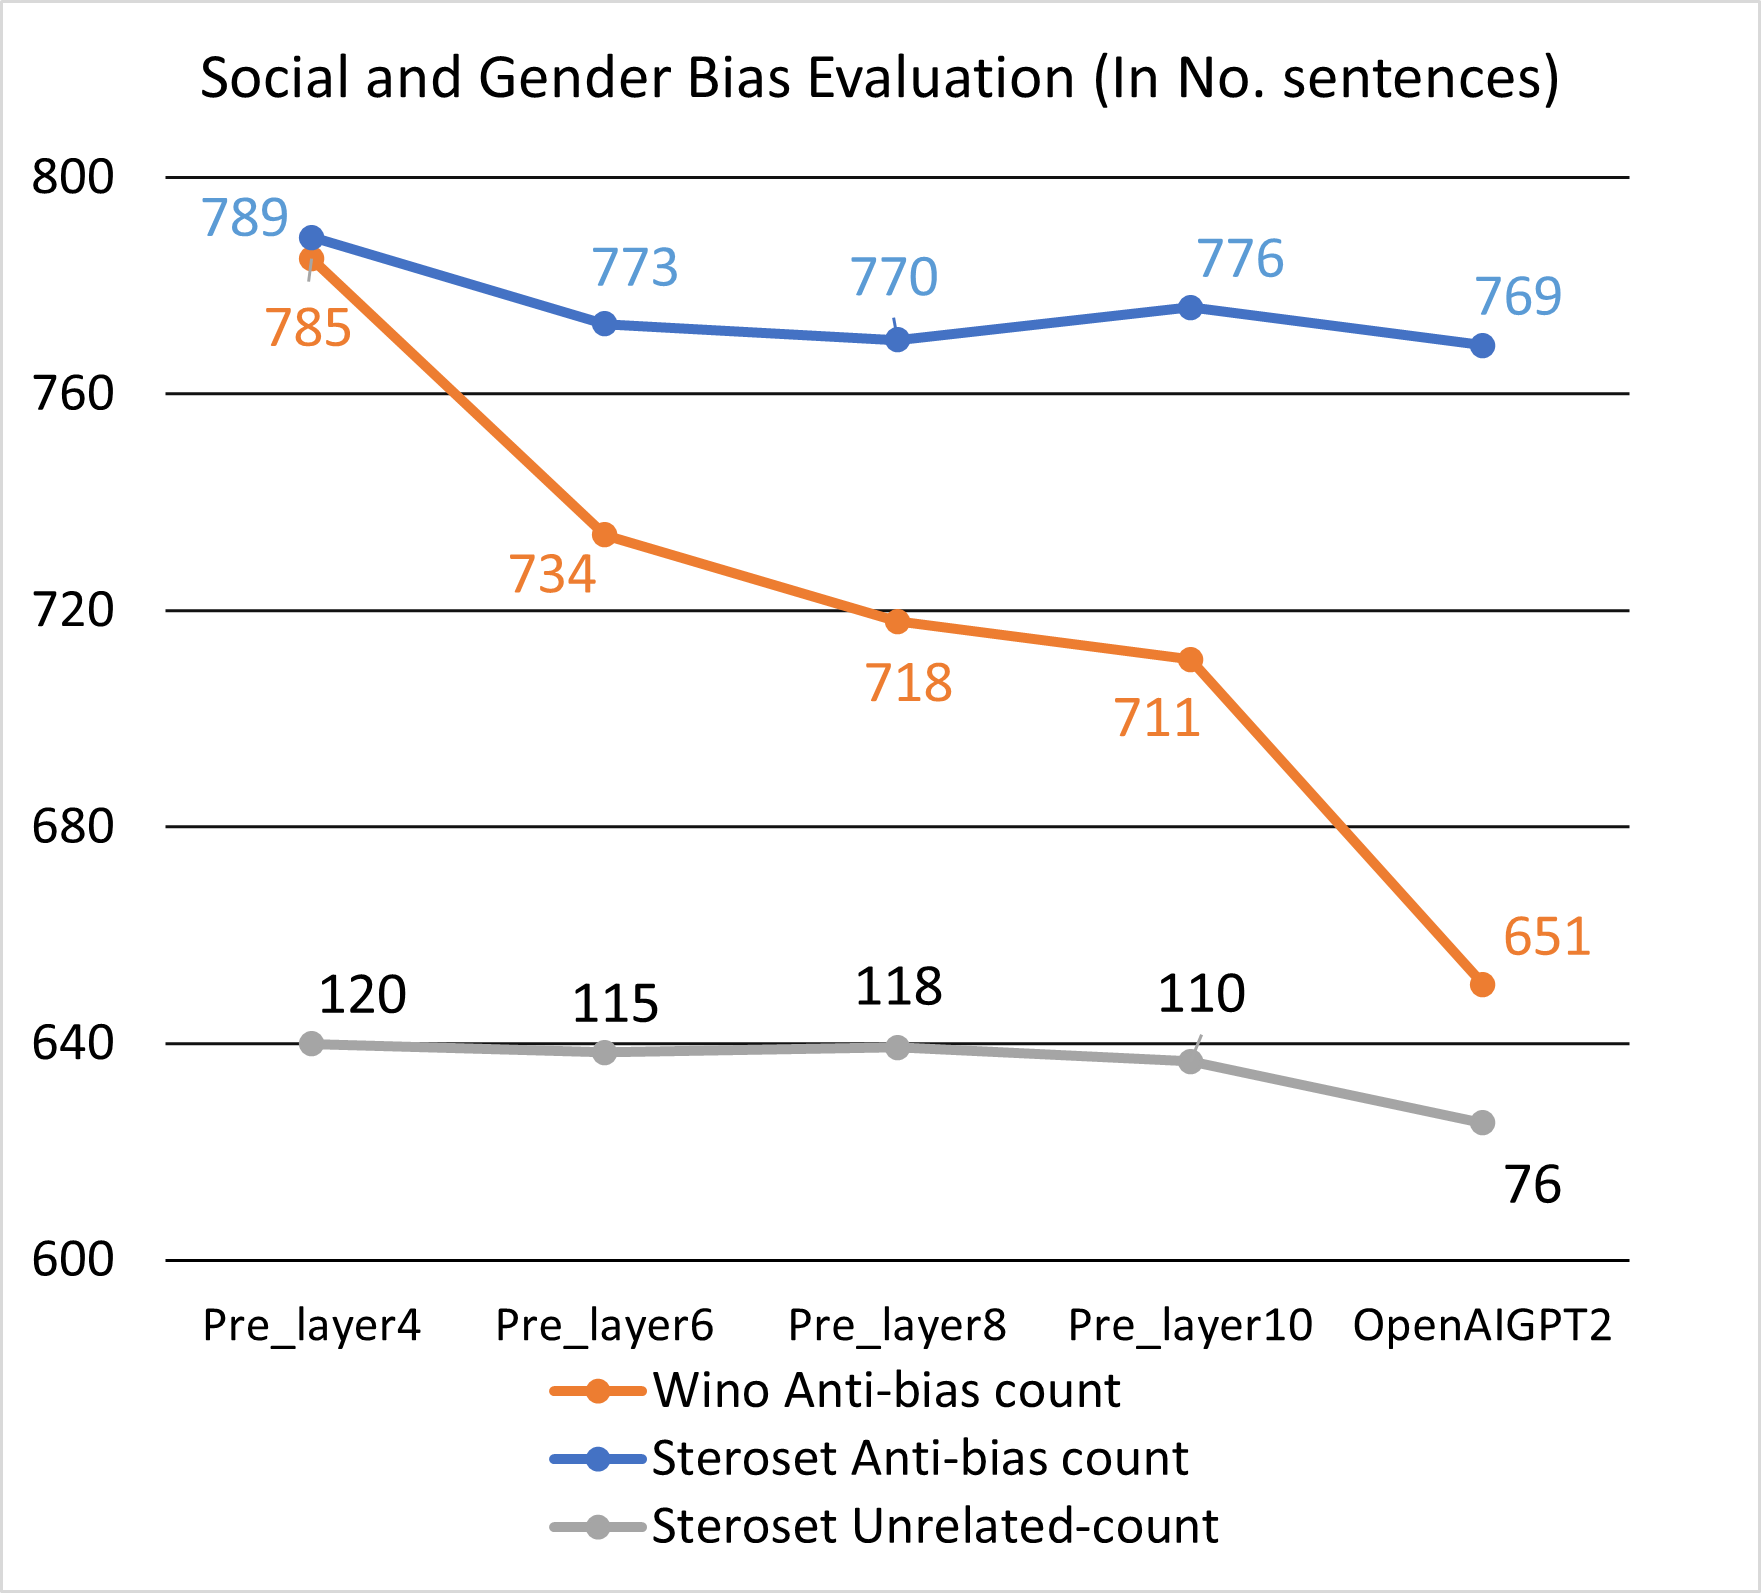
\includegraphics[scale = 0.57]{graphs/social_bias_2.png}
\caption{Stereoset Bias}
\centering
\label{fig: stereobias}
\end{figure}

\subsection{Bias in Model Generation}


\noindent \textbf{Stereoset} \quad We first test the models on the Stereoset dataset, which was specifically curated by \cite{Nadeem2021StereoSetMS} to measure social bias in language models. For each model, we plot the total number of times that it chooses anti-stereotype word and unrelated words. The more anti-stereotypes it chose, the less biased it is. And the more unrelated words it choose, the more unreliable it is. The result is shown in Figure \ref{fig: stereobias}.\\


\noindent \textbf{Winobias} \quad Winobias dataset has a similar format as Stereoset, and is used to measure gender bias. It contains a total of 1584 samples, and we count the number of times each model chooses anti-bias sentences. For both datasets, the more anti-stereotypes it chose, the less biased it is. The result is shown in Figure \ref{fig: stereobias}. Other papers \cite{Barikeri2021RedditBiasAR} calculate mean perplexity difference between the anti-bias and biased sentences to measure the bias level of language models; however,since there's a significant inequality in the original perplexity of different models we compare, mean perplexity difference can be directly applied to our setting. \\

\noindent \textbf{Observation} \quad We find that gender bias level consistently decrease as the model size becomes smaller; but distillation's the effect on Stereoset dataset isn't obvious. The current experiment may be too weak to give any convincing conclusion now, but there does seem to be a trend of bias reduction after distillation.


\subsection{Ablation Study}

We conduct an ablation study to mitigate the concern that toxicity reduction is only the result of smaller model size. As in Figure \ref{fig: Ablation}, the DialoGPT \cite{Zhang2020DIALOGPTL} models (small, medium, large) are publicly available pretraiend models on Huggingface, trained from scratch using different architectures, rather than being distilled. The trend of toxicity and bias reduction is not observed in the DialoGPT models. Rather, toxicity decreases is observed in Distilled-400M Blenderbot versus orginal Blenderbot 3B. This study confirms that it's distillation, rather than simple model size that causes the observed fairness pattern. \\

\begin{figure}[ht!]
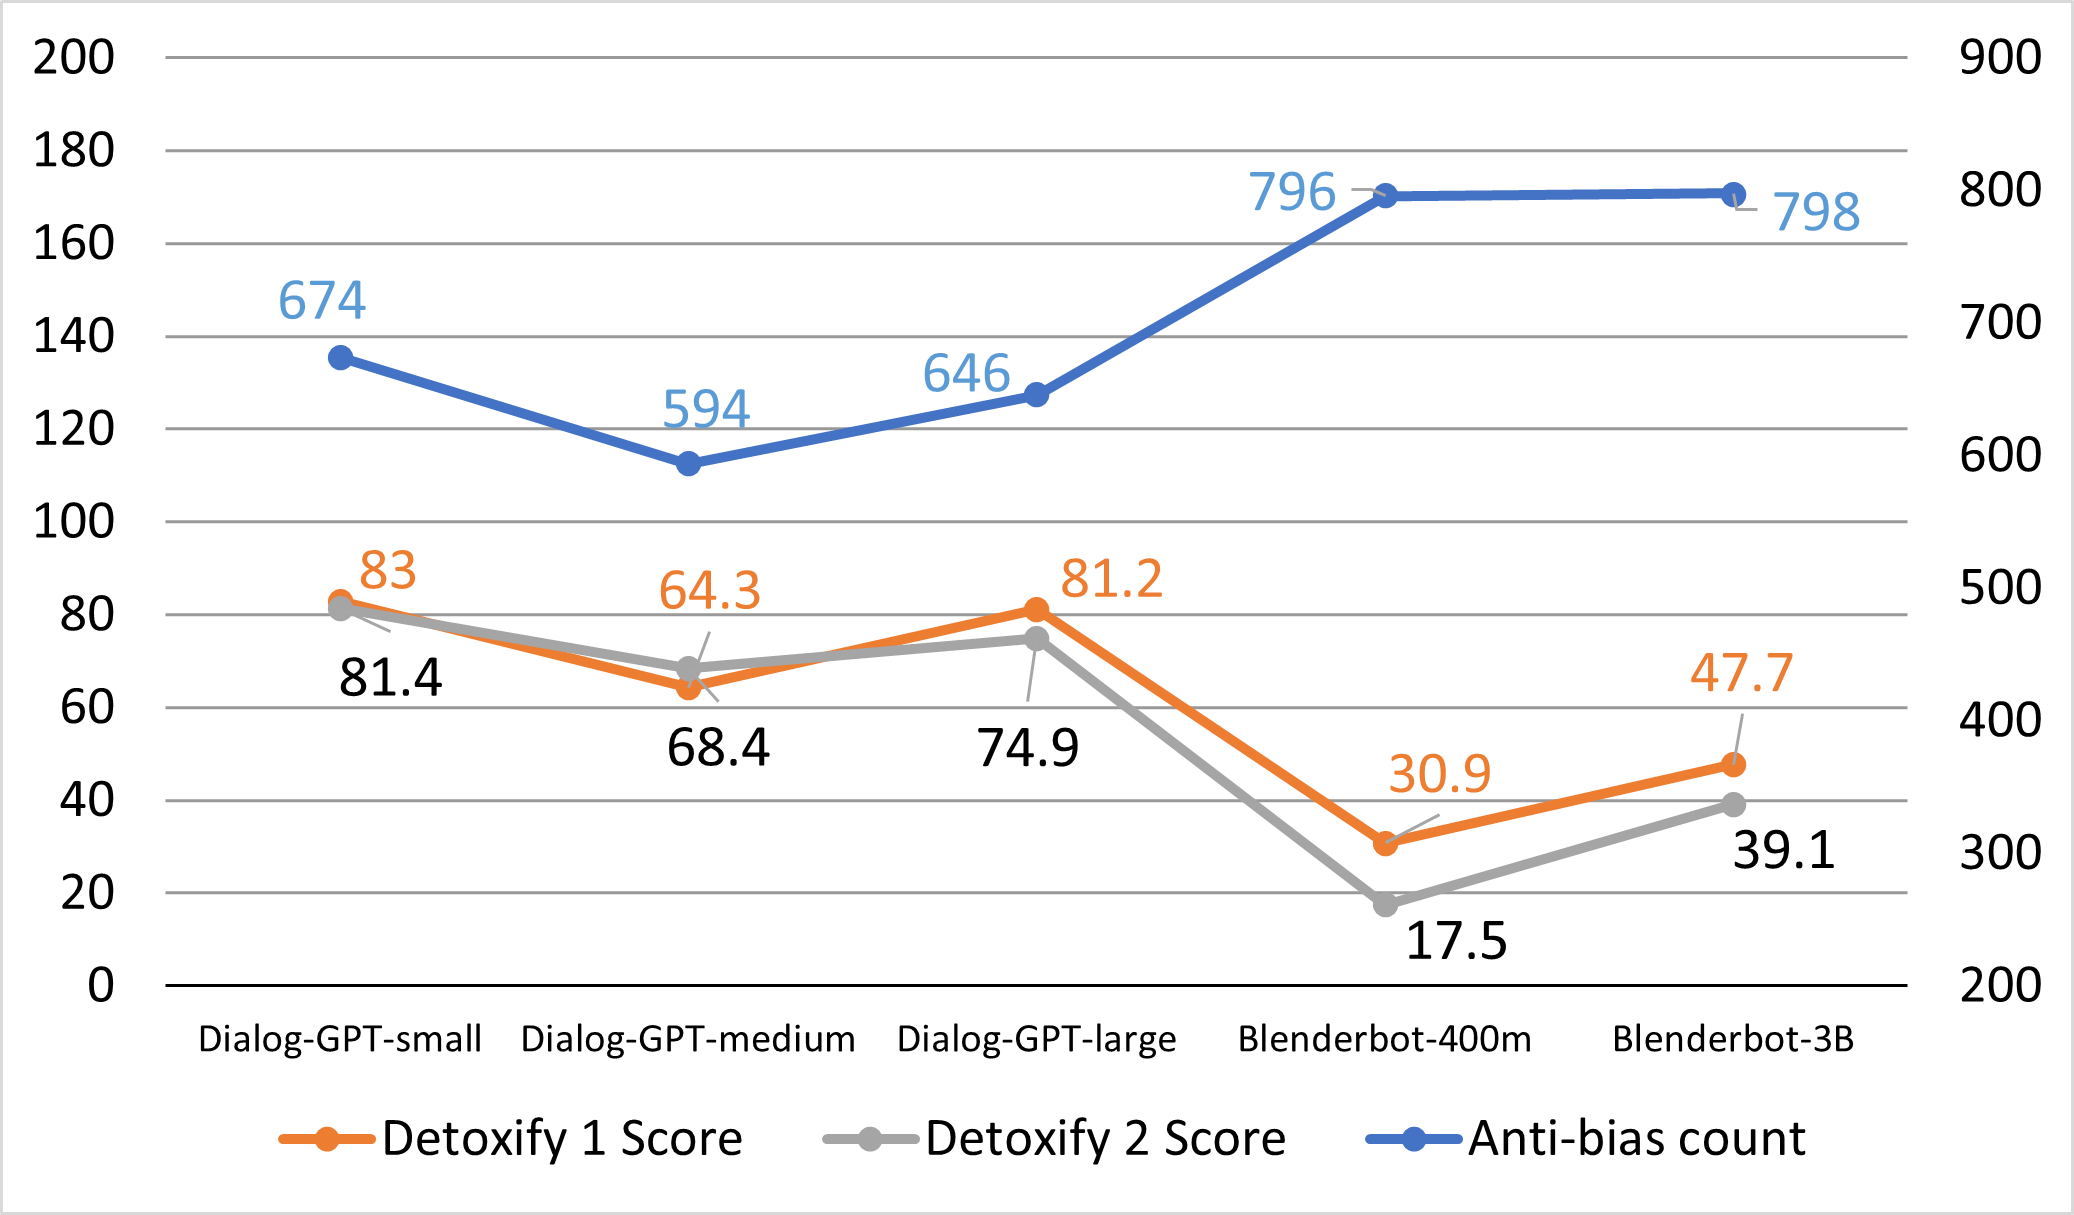
\includegraphics[scale = 0.48]{graphs/bias_toxicity.png}
\caption{Ablation Study}
\centering
\label{fig: Ablation}
\end{figure}


\subsection{Perplexity vs Bias $/$ Toxicity}

Figure \ref{fig: ppl_bias_t} illustrates a potential weakness of our experiments; that is as the PPL decreases, model toxicity and bias level increases. Then, it can be argued that it's low perplexity that caused models to seem less biased and less toxic. However, in general, it's difficult to match heavily compressed model's PPL with the original model, so this concern couldn't be easily addressed. What we can do in the future is to narrow down the perplexity differences, and observe if there's any decrease in bias/toxicity reduction. 

\begin{figure}[ht!]
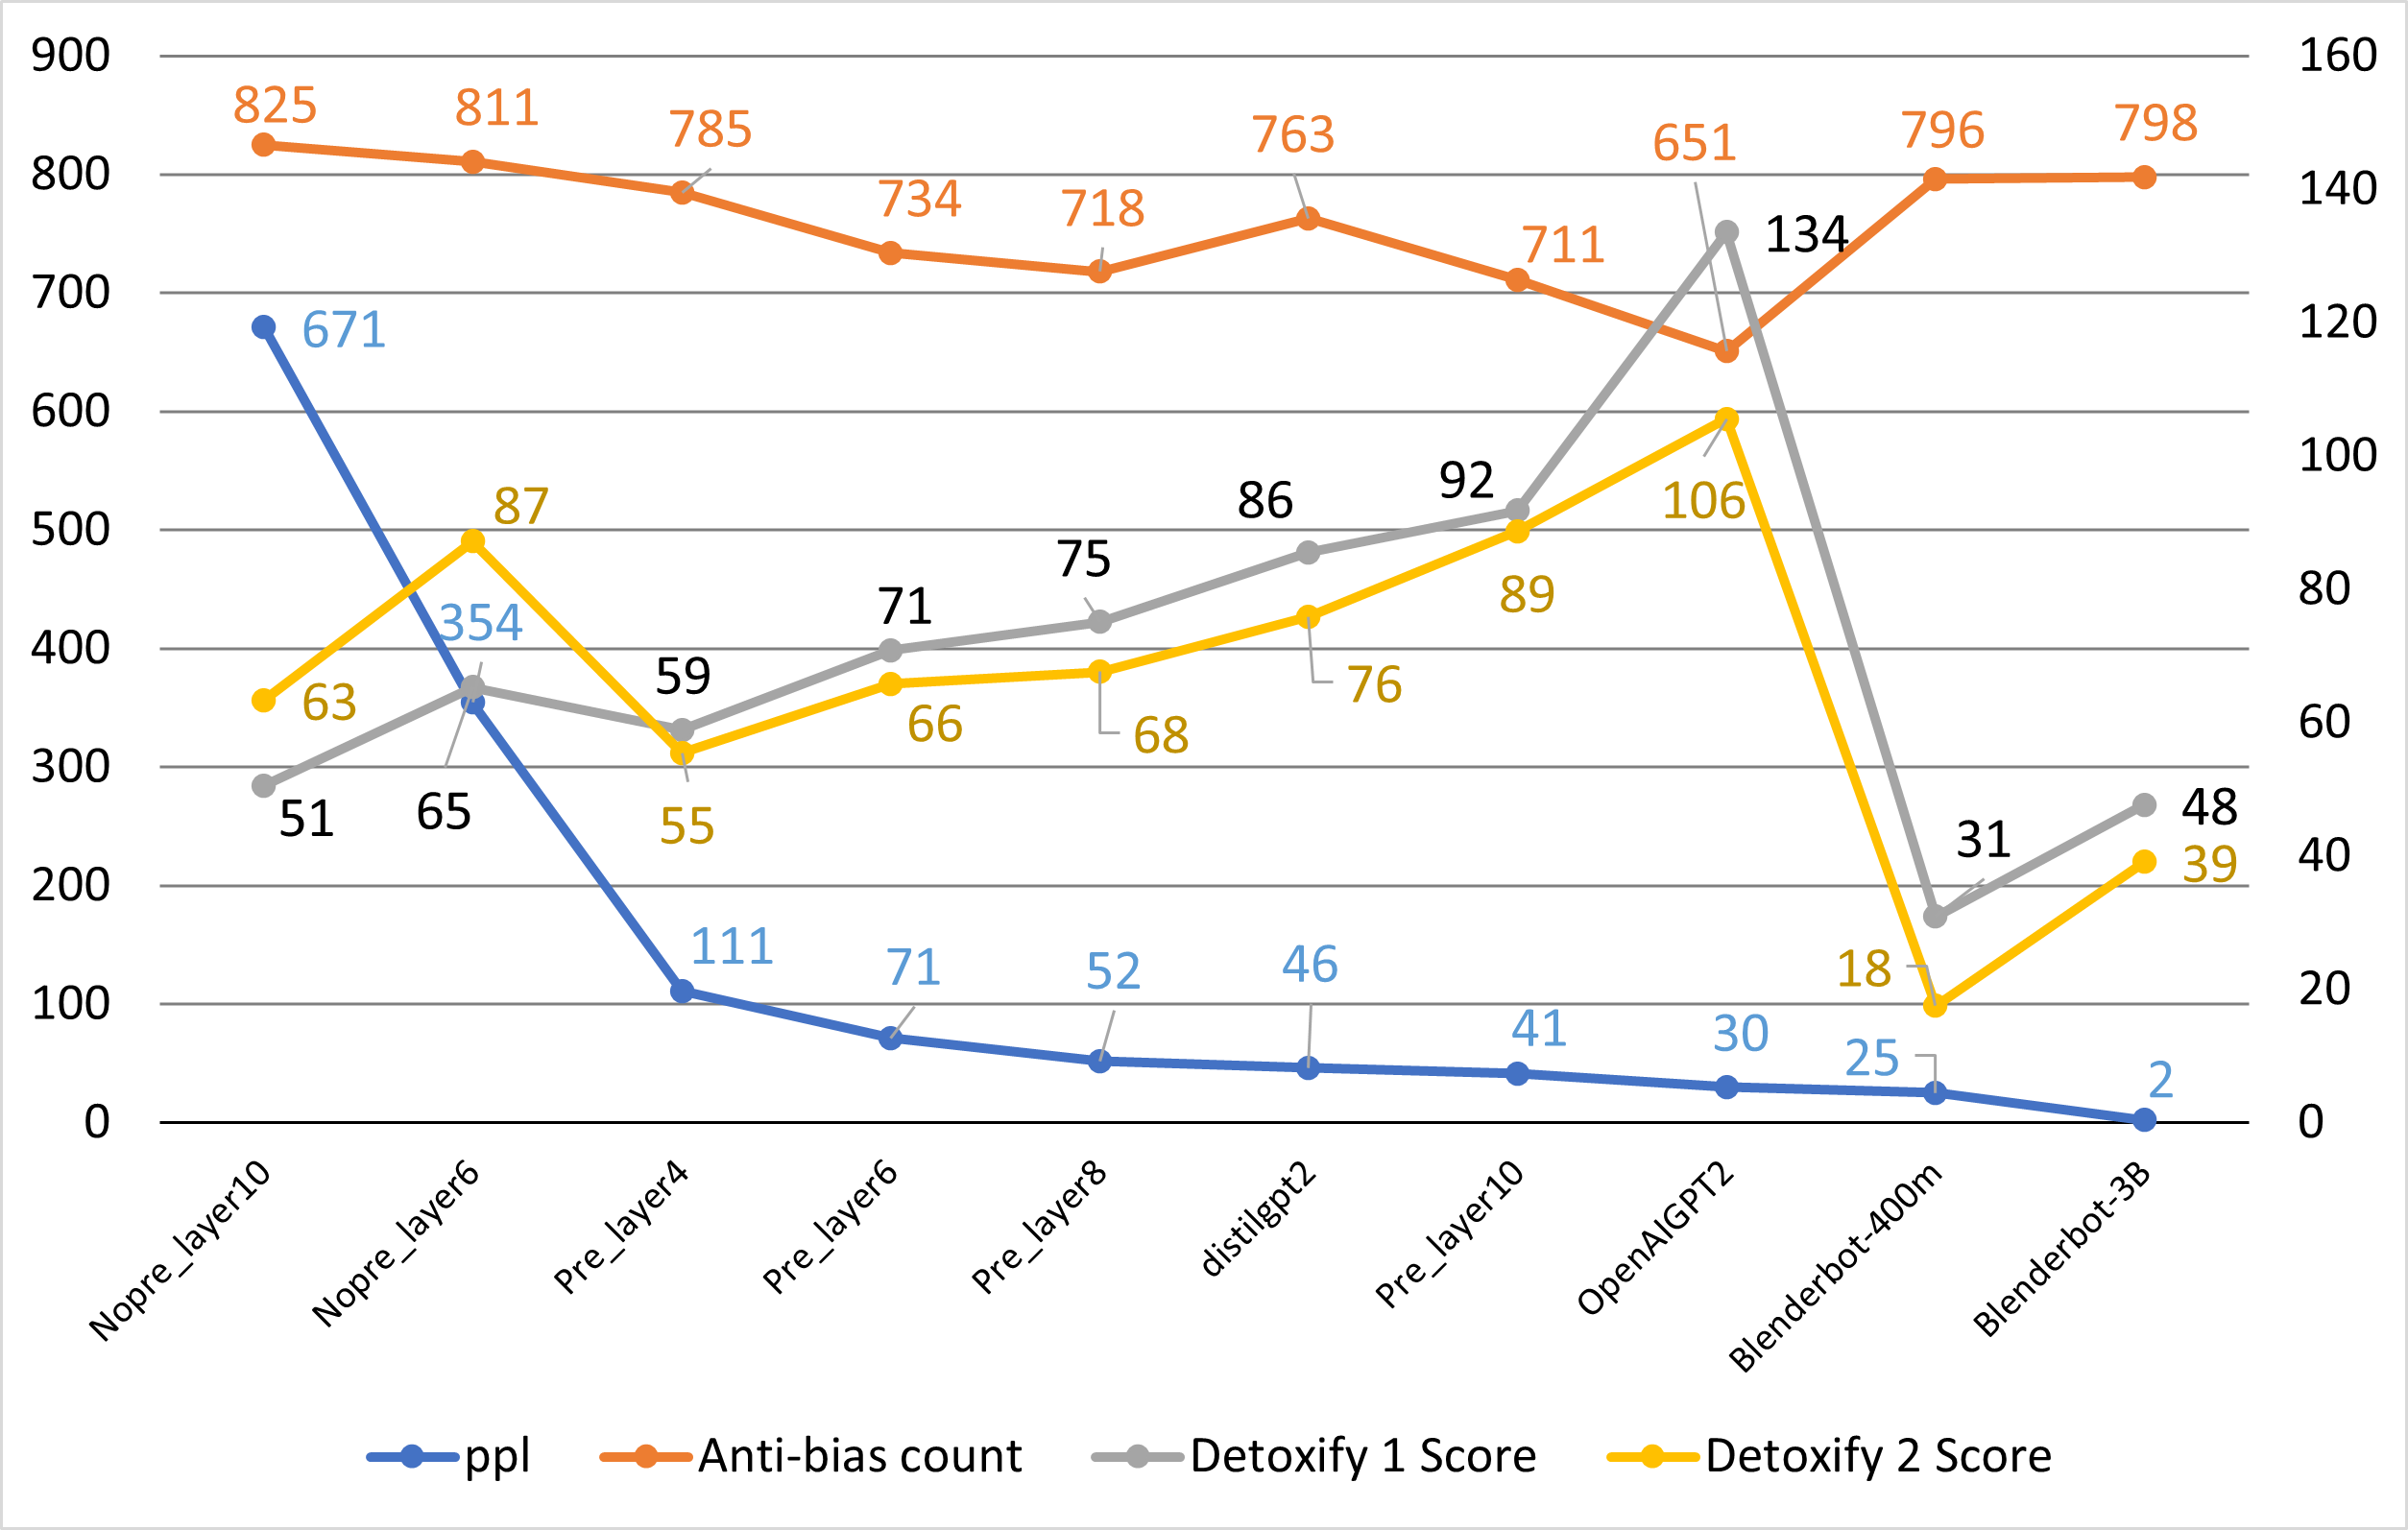
\includegraphics[scale = 0.4]{graphs/ppl_bias_toxicity.png}
\caption{Perplexity vs Bias $/$ Toxicity}
\centering
\label{fig: ppl_bias_t}
\end{figure}


